\documentclass{article} 
\usepackage{polski} 
\usepackage[utf8]{inputenc} 
\usepackage[OT4]{fontenc} 
\usepackage{graphicx,color} 
\usepackage{url}
\usepackage{float}
\usepackage[pdftex,hyperfootnotes=false,pdfborder={0 0 0}]{hyperref} %za wszystkimi pakietami; pdfborder nie wszedzie tak samo zaimplementowane bo specyfikacja nieprecyzyjna; pod miktex'em po prostu nie widac wtedy ramek

% Zmiana rozmiarów strony tekstu
\addtolength{\voffset}{-1cm}
\addtolength{\hoffset}{-1cm}
\addtolength{\textwidth}{2cm}
\addtolength{\textheight}{2cm}

%bardziej zyciowe parametry sterujace rozmieszczeniem rysunkow
\renewcommand{\topfraction}{.85}
\renewcommand{\bottomfraction}{.7}
\renewcommand{\textfraction}{.15}
\renewcommand{\floatpagefraction}{.66}
\renewcommand{\dbltopfraction}{.66}
\renewcommand{\dblfloatpagefraction}{.66}
\setcounter{topnumber}{9}
\setcounter{bottomnumber}{9}
\setcounter{totalnumber}{20}
\setcounter{dbltopnumber}{9}

% własny bullet list z malymi odstepami
\newenvironment{tightlist}{
\begin{itemize}
  \setlength{\itemsep}{1pt}
  \setlength{\parskip}{0pt}
  \setlength{\parsep}{0pt}}
{\end{itemize}}

%obrazkow szukamy w nastepujacym katalogu:
\graphicspath{{pics/}}



%\title{Sprawozdanie z laboratorium:\\Metaheurystyki i Obliczenia Inspirowane Biologicznie}
%\author{}
%\date{}


\begin{document}

\thispagestyle{empty} %bez numeru strony

\begin{center}
{\large{Sprawozdanie z laboratorium:\\
Uczenie Maszynowe i Sieci Neuronowe}}

\vspace{3ex}


\vspace{3ex}
{\footnotesize\today}

\end{center}


\vspace{10ex}

Prowadzący: dr hab.~inż. Maciej Komosiński

\vspace{5ex}

Autorzy:
\begin{tabular}{lllr}
\textbf{Maciej Trojan} & inf94378 & ISWD & maciek.trojan@me.com \\
\textbf{Paweł Rychły } & inf94362 & ISWD & pawelrychly@gmail.com \\
\end{tabular}

\vspace{5ex}

Zajęcia środowe, 11:45.


\newpage


\section{Uczenie nadzorowane sztucznych sieci neuronowych}

\paragraph{Zadanie 2. Różnice funkcjonalne pomiędzy sieciami jedno- i wielowarstwowymi oraz pomiędzy sieciami liniowymi a nieliniowymi (uczenie sieci warstwowych funkcji logicznej AND i funkcji różnicy symetrycznej XOR)}

\subparagraph{1. Skonstruuj zbiór przykładów definiujący dwuargumentową funkcję ("bramkę") AND (File|New|Data set) i zachowaj go. Wszystkie 4 przykłady mają stanowić zbiór uczący. Jakie są klasy decyzyjne w tym zbiorze przykładów i jakie są ich liczności?\\}

Zbiór zawiera dwie klasy decyzyjne: 1 i 0. Ich liczności wynoszą odpowiednio: 1 i 3. 

\begin{table}[h]
    \begin{tabular}{|c|c|c|}
     \hline
     	VAR1 & VAR2 & decyzja \\ \hline
        0 & 0 & 0 \\ 
        0 & 1 & 0 \\ 
		1 & 0 & 0 \\ 
		1 & 1 & 1 \\ \hline             
    \end{tabular}
    \caption{Zbiór przykładów uczących}
\end{table} 

\subparagraph{3. Wyobraź sobie (narysuj) pożądaną funkcję odpowiedzi sieci (trójwymiarowy wykres zależności wyjścia od dwóch wejść)\\}

\begin{figure}[H]
\begin{center}
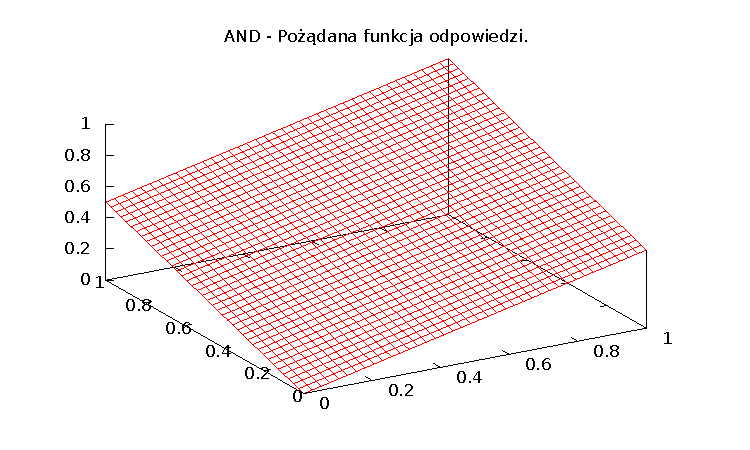
\includegraphics[width=1\textwidth]{pozodana_funnkcja_odpowiedzi_and.pdf}
\end{center}
\caption{Pożądana funkcja odpowiedzi sieci}
\label{fig-1Tdelta}
\end{figure}

\subparagraph{4. Skonstruuj liniową sieć jednowarstwową o architekturze 2-1 (File|New|Network, Type=Linear, przycisk Advise). Uaktywnij okno wykresu błędu średniokwadratowego (Statistics|Training graph). Naucz sieć na problemie AND (Train|Multilayer perceptron|Back propagation). Obejrzyj funkcję odpowiedzi sieci (Run|Responce surface) i błędy dla poszczególnych przypadków (Statistics|Case errors)\\}

\begin{figure}[H]
\begin{center}
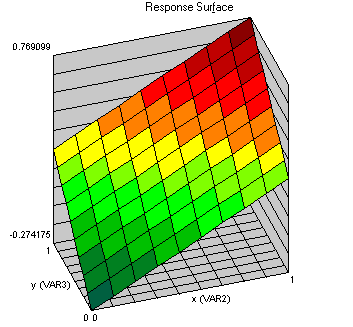
\includegraphics[width=0.5\textwidth]{And-training-3D.png}
\end{center}
\caption{Funkcja odpowiedzi sieci}
\label{fig-1Tdelta}
\end{figure}

\begin{figure}[H]
\begin{center}
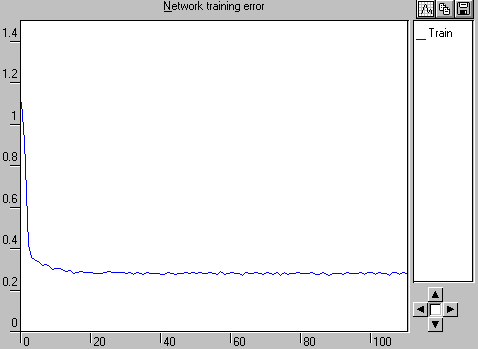
\includegraphics[width=0.5\textwidth]{And-training-Error.png}
\end{center}
\caption{Wykres błędu}
\label{fig-1Tdelta}
\end{figure}

\begin{figure}[H]
\begin{center}
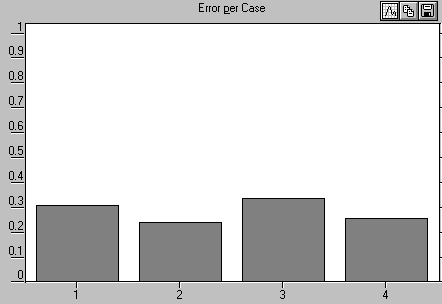
\includegraphics[width=0.5\textwidth]{And-training-CaseError.png}
\end{center}
\caption{Błędy dla poszczególnych przypadków}
\label{fig-1Tdelta}
\end{figure}


\end{document}

